\documentclass[12pt,letterpaper]{article}

\usepackage{amsmath} 
\usepackage{amssymb}
\usepackage{ulem}
\usepackage{tikz}
\usetikzlibrary{positioning,shapes.misc}
\usepackage[left=1in,top=1in,right=1in,bottom=1in,nohead]{geometry}

\usepackage{amsthm} 
\newtheorem{mydef}{Definition}
\newtheorem{example}{Example}
\newtheorem{thrm}{Theorem}
\newtheorem{lemma}{Lemma}
\newtheorem{cor}{Corollary}
\newcommand{\biu}[1]{\underline{\textbf{\textit{#1}}}}
\newcommand{\so}{\Rightarrow}
\usepackage[ampersand]{easylist}

\colorlet{circle edge}{gray!50}
\colorlet{circle area}{gray!20}

\tikzset{filled/.style={fill=circle area, draw=circle edge, thick},
    outline/.style={draw=circle edge, thick}}

\begin{document}

\begin{figure}
\label{piston}
\begin{center}
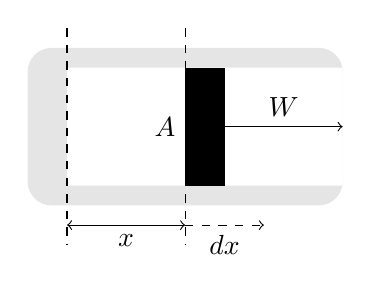
\begin{tikzpicture}[auto]
\begin {scope}
	\fill [filled, rounded corners=2ex] (0,0) rectangle (4,2) 
	[filled, draw=none, even odd rule, rounded corners=0ex] (0.5,0.25) rectangle (4,1.75);
	\fill (2,0.25) rectangle (2.5,1.75);
	\draw[left] node at (2,1) {$A$};
	\draw[->] (2.5,1) -- (4,1) ;
	\draw[above] node at (3.25,1) {$W$};
	\draw[dashed] (0.5,2.25) -- (0.5,-0.5);
	\draw[dashed] (2,2.25) -- (2,-0.5);
	\draw[<->]  (0.5,-0.25) -- (2,-0.25);
	\draw[below] node at (1.25,-0.25) {$x$};
	\draw[->,dashed] (2,-0.25) -- (3,-0.25);
	\draw[below] node at (2.5,-0.25) {$dx$};
\end{scope}
\end{tikzpicture}
\end{center}
\caption{Piston}
\end{figure}

Consider the depicted isolated piston in figure \ref{piston}. There is no heat exchange between the (ideal) gas inside and the outside world, but the piston does some work $W$. 

Before analyzing the problem it may be useful to identify which variables and constants are involved and what equations will be useful in solving the problem. Since we are assuming the inside to be an ideal gas, we can make use of the following equations:
\begin{eqnarray*}
	pV &=& nRT\\
	pV &=& \frac{2}{3}U
\end{eqnarray*}

In these equations $R$ is a constant as always and so is $n$, because no molecules can escape from the piston. However, since the piston is not thermically  connected to the outside world $T$ may or may not be constant and we will therefore treat is as a variable. $p$,$V$ and $U$ will be variables as well as we are used to from previous problems.

Now, to begin analyzing the problem let us use first determine the change in internal energy ($U$) of the gas. By the conservation of energy, we must clearly have.
\[ U = W + U' \]
where $W$ is the work done by the piston and $U'$ is the amount of internal energy. Recall the $p=\frac{F}{A}$ and that we may thus represent the work done (and thus  negative change in internal energy) for an infinitesimal movement $dx$ of the piston as 
\[ dU=-pAdx \].
The change in volume of the inside of the piston is given by 
\[ dV=Adx \].
We are now ready to proceed by making use of the equation 
\[ pV = \frac{2}{3}U \]
Taking the differentials (if you haven't seen this before, just consider this a time derivative multiplied by $dt$ on both sides) yields
\[ pdV + Vdp = \frac{2}{3} dU \]
and by plugging in $dV$ and $dU$ from above we get
\[ pAdx + Vdp = -\frac{2}{3} pAdx \]
which simplifies to
\[ \frac{dp}{p} = -\frac{5}{3}\frac{Adx}{V} \]
Now notice that since $V=Ax$, $dV=Adx$ and thus we may write the equation as 
\[ \frac{dp}{p} = -\frac{5}{3}\frac{dV}{V} \]
Integrating both sides gives 
\[ \ln(p) = -\frac{5}{3}\ln(V) + C_1 \]
or
\[ \ln(p) = \ln\left(\frac{1}{V^{5/3}}\right)+C_1 \]
and by taking the exponent of both sides we find
\[ p = \frac{C}{V^{5/3}} \]
\[ pV^{5/3} = const. \]

\end{document}
